\section{Benchmarks}
\begin{figure}
    \centering
    \subfigure{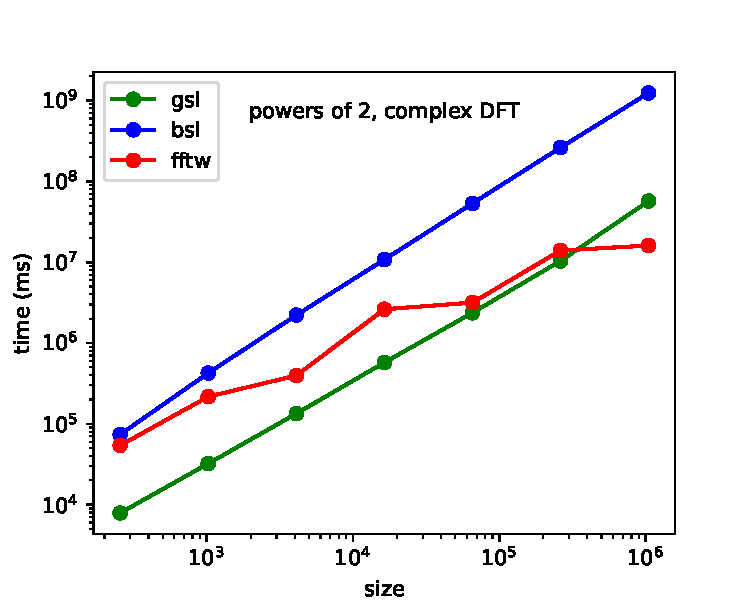
\includegraphics[width=0.49\textwidth]{plots/complex_p2.pdf}}
    \subfigure{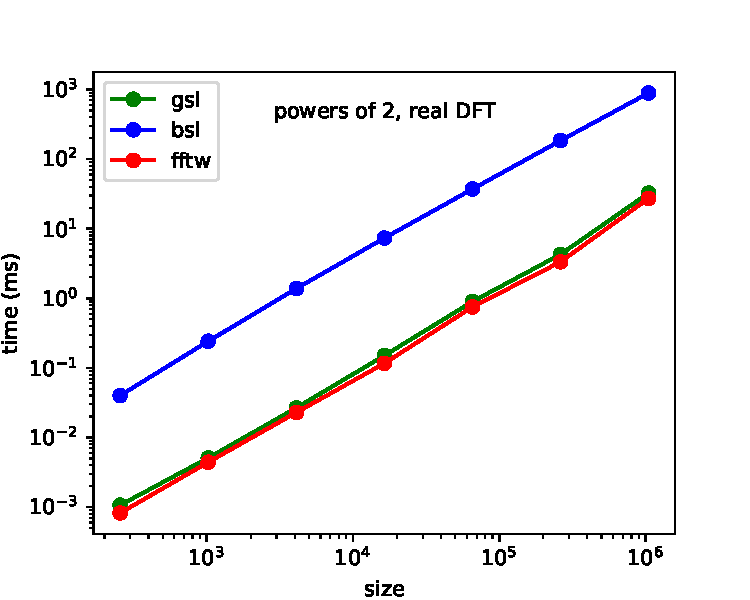
\includegraphics[width=0.49\textwidth]{plots/real_p2.pdf}}
    \vfill
    \subfigure{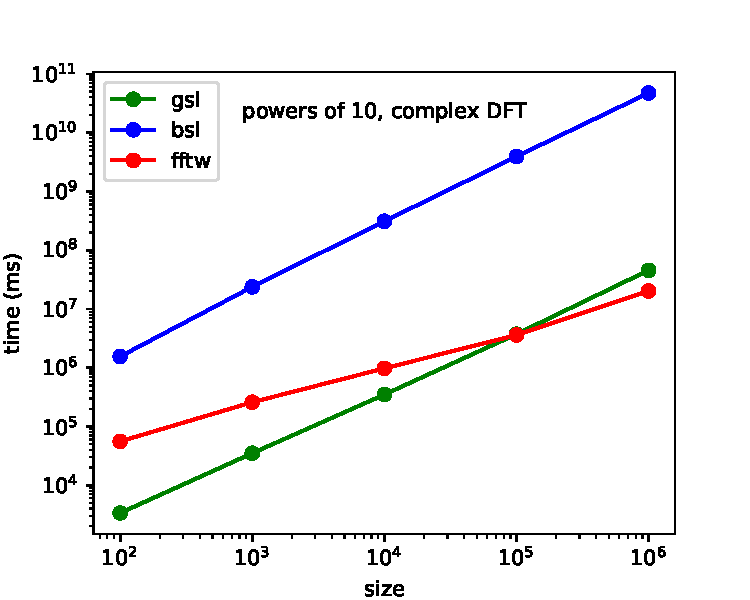
\includegraphics[width=0.49\textwidth]{plots/complex_p10.pdf}}
    \subfigure{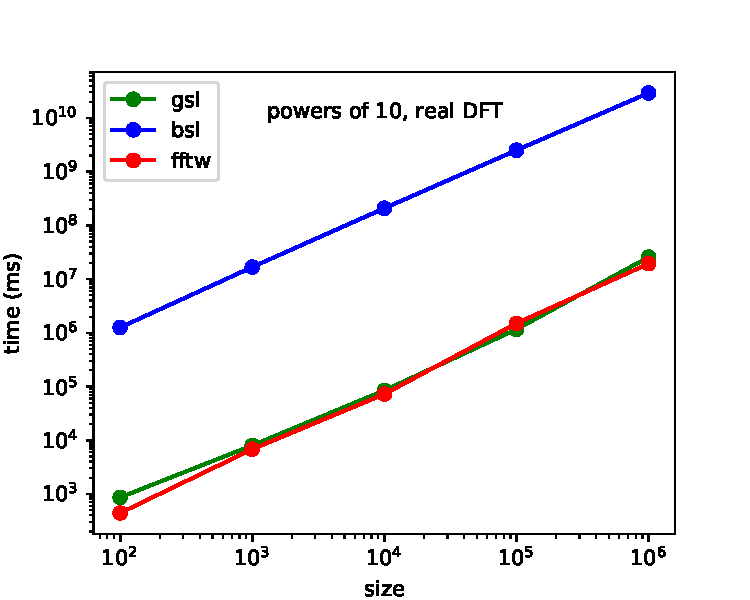
\includegraphics[width=0.49\textwidth]{plots/real_p10.pdf}}
    \vfill
    \subfigure{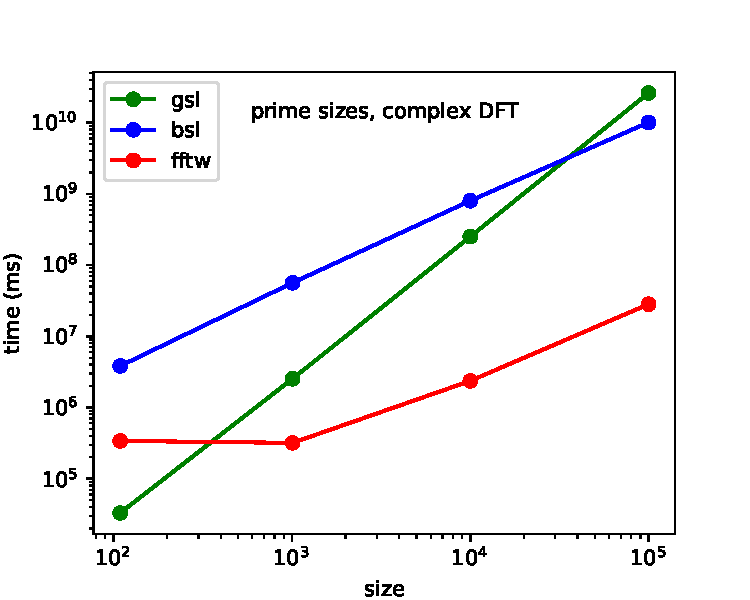
\includegraphics[width=0.49\textwidth]{plots/complex_primes.pdf}}
    \subfigure{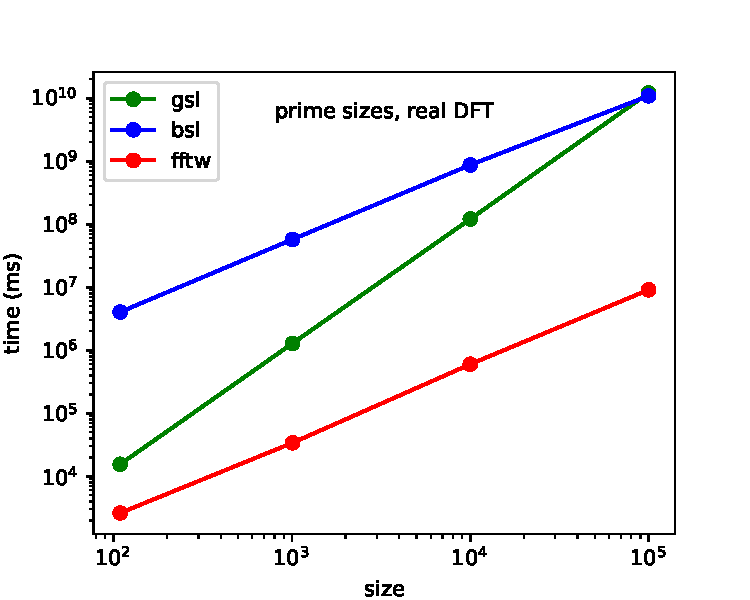
\includegraphics[width=0.49\textwidth]{plots/real_primes.pdf}}
    \caption{Benchmarks for different DFT sizes (rows), complex and real
    algorithms (columns), for our three backends: BSL, GSL and FFTW.}
\end{figure}

%\begin{figure}
%   \centering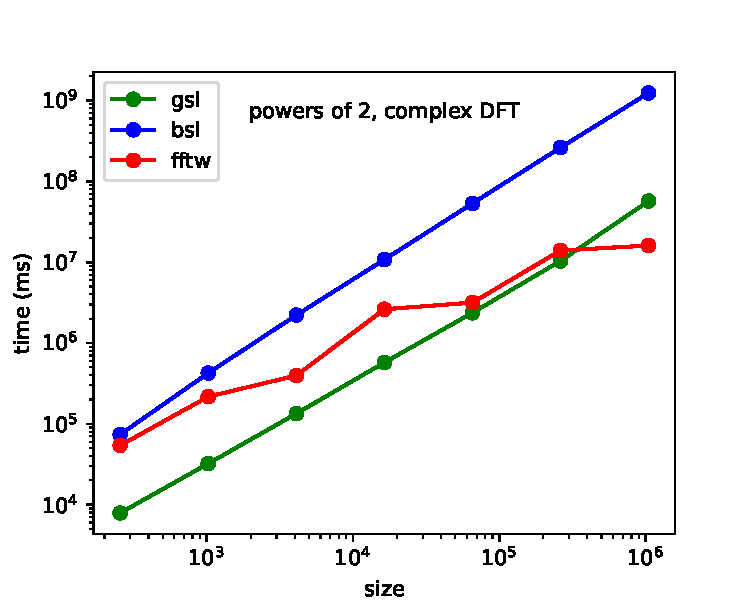
\includegraphics{plots/complex_p2.pdf} 
%   \caption{Benchmarks for powers of 2 sizes, double precision complex data.}
%\end{figure}
%\begin{figure}
%   \centering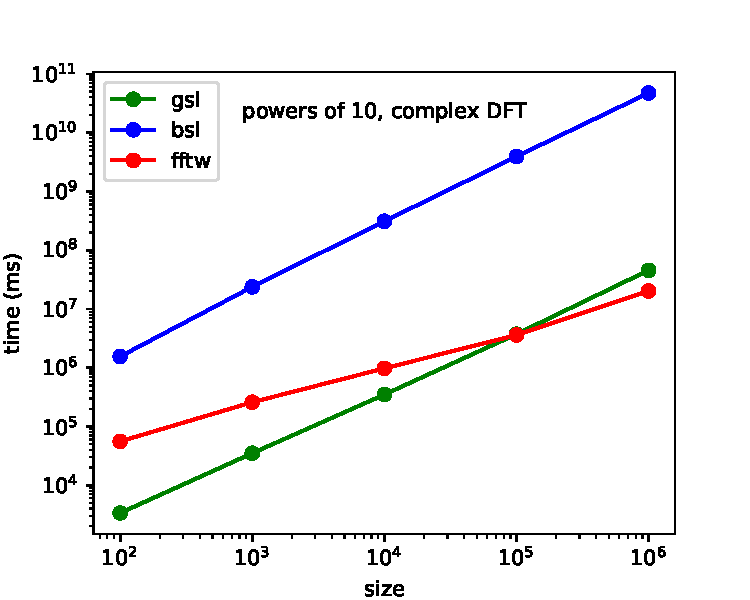
\includegraphics{plots/complex_p10.pdf} 
%   \caption{Benchmarks for powers of 10 sizes, double precision complex data.}
%\end{figure}
%\begin{figure}
%   \centering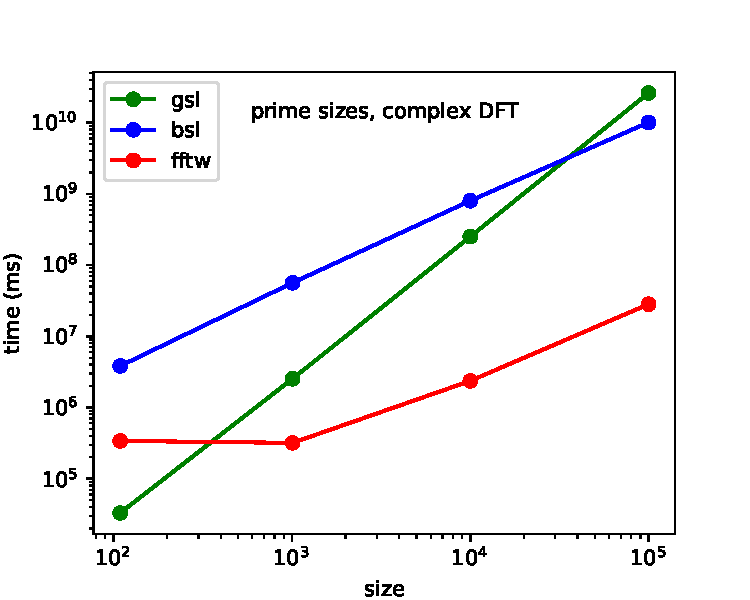
\includegraphics{plots/complex_primes.pdf} 
%   \caption{Benchmarks for prime sizes, double precision complex data.}
%\end{figure}
%
%\begin{figure}
%   \centering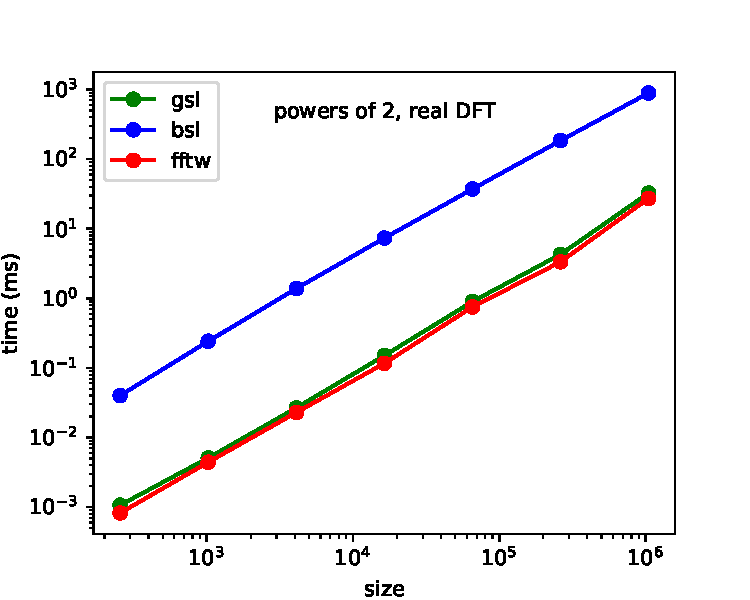
\includegraphics{plots/real_p2.pdf} 
%   \caption{Benchmarks for powers of 2 sizes, double precision real data.}
%\end{figure}
%\begin{figure}
%   \centering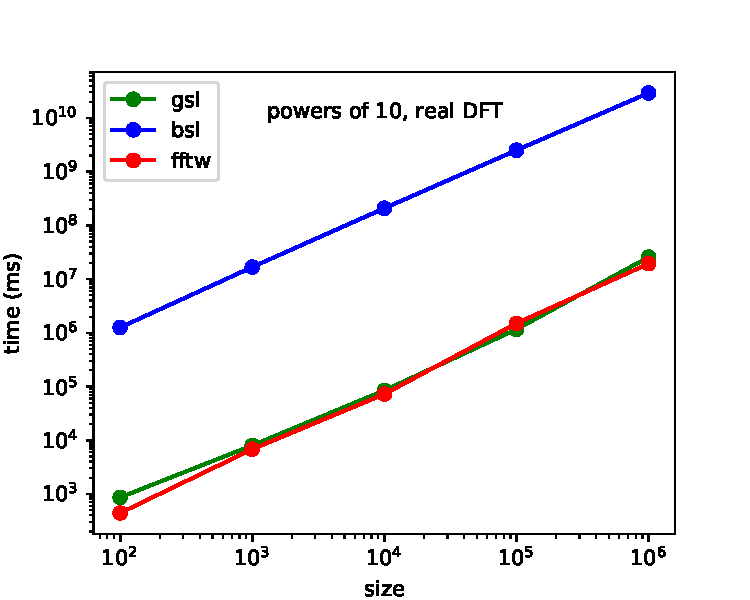
\includegraphics{plots/real_p10.pdf} 
%   \caption{Benchmarks for powers of 10 sizes, double precision real data.}
%\end{figure}
%\begin{figure}
%   \centering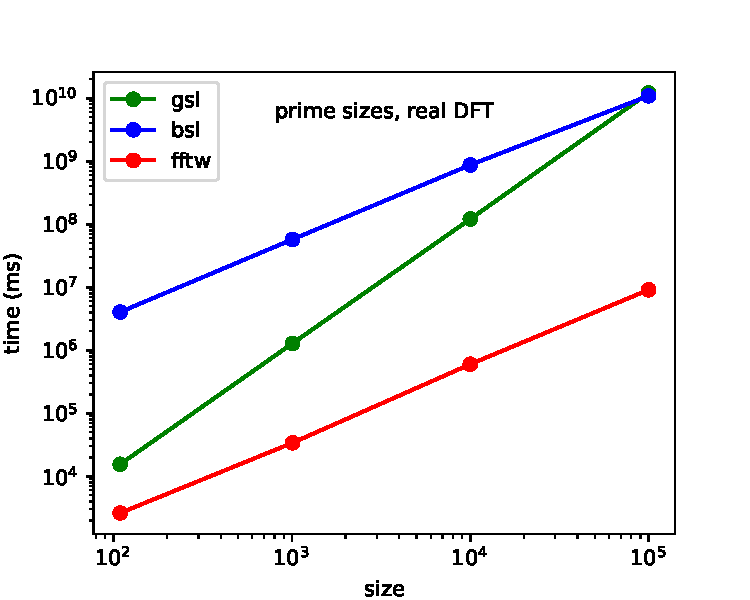
\includegraphics{plots/real_primes.pdf} 
%   \caption{Benchmarks for prime sizes, double precision real data.}
%\end{figure}
